% create a diagram how network namespaces work
% remember we are still a non-root? Let's apply tc.
% add namespace stuff to the container script
% tc qdisc add dev eth0 root netem delay 100ms

% To begin with, I would like to start with the conclusions. Devil hides in the
% details. And those details are worth hundreds of millions of dollars.

% And now let's dive deep into this. A lot of people use Docker/rkt (how many
% of you?), but very often we do not have time to actually understand how they
% work. So today in half-hour I will show you in a nutshell how that works. My
% hope is that even after you know how to build a container engine, I can still
% convince you that the existing tools are worth spending $MM to create and use.

% End: I created, but look at my conclusions again.

% 22.40
% Jau is esmes gali pristatyti, bet, pataisius detales, bus daug patraukliau ;)
% Patiko pradzia apie tavo patirti
% Pradzioj – tai ka tu is esmes pasakosi/darysi ir kodel tai man gali buti aktualu?
% Daug teksto, kuris yra toks pat ir skaidrej, ir tu ji atkartoji
% Uzsirasyk KONKRECIUS pavyzdzius, ka typinsi!! Kad tikrai veiktu!
% Pasiimk lazeriuka?
% Del nuolatinio typinimo prarandi kontakta su publika
% Pasakyk, ka darysi ir ko tikiesi. O tada pasakyk, kad «va, taip ir gavom«  (cia apie visus kodinimus)
% Didele dali paskaitos galvojau, bet gi as kodus galiu susirasti internete – man reikia daugiau izvalgu !
% Neatsidusk taip, tarsi butum pavarges ar butu nuobodu :P
% Ar suderintos tech galimybes ?
% Tai kokia isvada?
% Conclusions neatitinka turini – cia future suggestions.
% 23.15

\documentclass[14pt]{beamer}
\usetheme{default}
\usepackage{graphics}
\usepackage{array}
\usepackage{verbatim}
\usepackage{hyperref}
\usepackage{biblatex}
\usepackage{tabularx}
\usepackage{soul}
\usepackage{mdframed}
\usepackage{tikz}
\usepackage{adjustbox}
\usepackage{mathtools}
\usepackage{caption}
\usepackage{fancyvrb}
\usepackage{subcaption}
\captionsetup{compatibility=false}

\usetikzlibrary{arrows,decorations.pathmorphing,backgrounds,positioning,fit,petri}

\definecolor{uberblack}{RGB}{9,9,26}
\definecolor{uberwhite}{RGB}{192,192,200}
\definecolor{uberblue}{RGB}{31,186,214}
\definecolor{darkgreen}{RGB}{32,96,32}
\setbeamercolor{title}{fg=uberblue}
\setbeamercolor{frametitle}{fg=uberblue}
\setbeamercolor{item}{fg=uberblue}
\setbeamercolor{navigation symbols dimmed}{fg=uberwhite}
\setbeamercolor{navigation symbols}{fg=uberwhite}

\hypersetup{linkcolor=}
\hypersetup{urlcolor=uberblue} % Does not apply color to href's
\hypersetup{colorlinks,urlcolor=uberblue} % href's are correct, but navigation links are magenta

\mode<presentation>{
    \setbeamertemplate{navigation symbols}{
        \insertslidenavigationsymbol
        \insertframenavigationsymbol
        \hspace{0.2cm}
        \begin{minipage}[c]{0.5cm}
            \vspace{-0.1cm}
            {\strut\insertframenumber{}/\inserttotalframenumber\strut}
        \end{minipage}
    }
}

\setbeamertemplate{footline}[text line]{%
\parbox{\linewidth}{
\vspace*{-8pt}\color{gray}
\textcircled{c}~2016. Uber Technologies Inc. All rights reserved.
}}

\newcommand{\framedgraphic}[2] {
    \begin{frame}{#1}
        \begin{center}
            \includegraphics[width=\textwidth,height=0.8\textheight,keepaspectratio]{#2}
        \end{center}
    \end{frame}
}

\newcommand{\withcredits}[3]
{
    \begin{minipage}[t][#1\textheight]{\textwidth}
        \vspace{5px}
        #2
    \end{minipage}
    \vfill
    \color{white}{\tiny Image source: #3}
}

%% =============================================================================

\title{Building blocks of Linux Containers}
\author{Motiejus Jak\v{s}tys \\
    motiejus@uber.com \\
    @mo\_kelione \\
    \vspace{1em}
    \includegraphics[height=1em]{media/svg_uberlogo.pdf}
}

\date{2016-11-18}

\begin{document}

\AtBeginSection[]
{
  \begin{frame}
    \frametitle{Table of Contents}
    \tableofcontents[currentsection]
  \end{frame}
}

\begin{frame}
\titlepage
\end{frame}

\section{Introduction}

\begin{frame}{Conclusion!}
    \pause
    Devil Hides in The Details\only<+>{.}\only<+->{?}
    \begin{itemize}[<+->]
        \item Many use Docker.
        \item We lack time to understand.
        \item Make container engine in 30 minutes.
        \item Details! \onslide<+->{$\rightarrow$ You will still pick existing tools.}
    \end{itemize}
\end{frame}

\subsection{Why me}
\begin{frame}{Why me}
    My resume: {\tiny oncall experience.}
    \begin{itemize}
        \item $2009-2012$ Telecom (Dev + Ops).
        \item $2012-2014$ Online Gaming (Dev + Ops).
        \item $2014-2016$ Amazon (Dev + Ops).
        \item $2016-now$ Uber (Dev + Ops):
            \begin{itemize}
                \item From $2016.02$: Dev.
                \item From $2016.11$: SRE.
            \end{itemize}
    \end{itemize}
    \onslide<+(1)->{I had to understand how exactly infrastructure works.}
\end{frame}

\subsection{A container in Linux is...}
\begin{frame}{A container in Linux is ...}
    \pause
    Fork/exec with bells \& whistles:
    \begin{itemize}[<+(1)->]
        \item Fancy tarball for distribution.
        \item COW filesystem to make it start fast.
        \item Cgroups for fairness.
        \item Namespaces for isolation.
    \end{itemize}
\end{frame}

\section{Namespaces}
\subsection{Isolation in Linux}
\begin{frame}{We will cover}
    \begin{itemize}[<+(1)->]
        \item User namespaces.
        \item Pid namespaces.
        \item Mount namespaces.
        \item Network namespaces.
        \item There are more, but not today.
    \end{itemize}
\end{frame}

\begin{frame}{User namespace}
    Become container-local root. \\
    {
        \tt unshare --map-root-user
    }
\end{frame}

\begin{frame}{Mount namespace}
    Hide container mounts. \\
    {
        \tt unshare --mount
    }
\end{frame}

\begin{frame}{Pid namespace}
    Hide other pids. \\
    {
        \tt unshare --pid --mount-proc --fork
    }
\end{frame}

\begin{frame}{Network namespace}
    Demonstrate this:
    \begin{itemize}[<+(1)->]
        \item Create namespace.
        \item Activate loopback ({\tt lo}).
        \item Create pair of devices {\tt veth1a} and {\tt veth1b}:
            \begin{itemize}
                \item {\tt veth1b} will go to the namespace.
                \item {\tt veth1a} will stay in default.
            \end{itemize}
        \item Add ip addresses.
        \item curl and ping.
        \item lsof, bind on ports separately.
    \end{itemize}
    \onslide<+(1)->{\small Ever wanted to run {\tt tcpdump} on an {\em application}?}
\end{frame}

\begin{frame}{Network namespace}
    \begin{adjustbox}{max totalsize={.9\textwidth}{.7\textheight},center}
        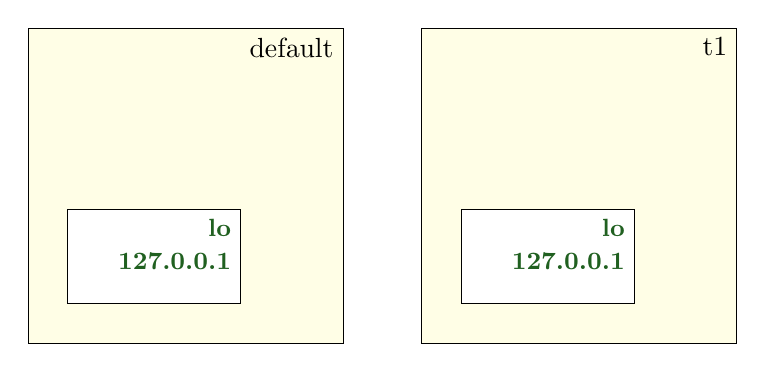
\begin{tikzpicture}
            \visible<+->{
                \filldraw[fill=yellow!10] (0,0) rectangle +(4,4) node[below left] { default };
                \filldraw[fill=white] (.5,.5) rectangle +(2.2,1.2) node[below left,align=right,text=darkgreen] { \bf \small lo \\ \bf \small 127.0.0.1 };
            }
            \visible<+->{
                \filldraw[fill=yellow!10] (5,0) rectangle +(4,4) node[below left] { t1 };
                \filldraw[fill=white] (5.5,.5) rectangle +(2.2,1.2) node[below left,align=right,text=red] { \bf \small lo \\ };
            }
            \visible<+->{
                \filldraw[fill=white] (5.5,.5) rectangle +(2.2,1.2) node[below left,align=right,text=darkgreen] { \bf \small lo \\ \bf \small 127.0.0.1 };
            }
        \end{tikzpicture}
    \end{adjustbox}
\end{frame}

\subsection{What did we just do}
\begin{frame}{What did we just do}
    \relax
    {\bf Created a container:}
    \begin{description}[<+(1)->]
        \item[User namespace] apt-get, iptables, mount, etc.
        \item[Isolated pids] no {\tt nobody}, isolate from each other.
        \item[Isolated mounts] e.g. for /tmp.
        \item[Isolated network] safely bind to {\tt :80}.
    \end{description}
    \onslide<+(1)->{An improvement over "run and hope it doesn't affect anything else".}
\end{frame}

\section{File systems and COW}
\begin{frame}{File systems and COW}
    A container:
    \begin{itemize}[<+->]
        \item Needs a file system.
        \item Starts quickly regardless of size.
    \end{itemize}

    \visible<+->{Do not want to copy 1GB with every startup.}

    \visible<+->{Copy On Write!}

    \visible<+->{\small lvm? zfs? btrfs?}
\end{frame}

\begin{frame}{A quick demo}
    \small
    \begin{itemize}
        \item Create {\tt tank/images/debian@latest}
        \item Create {\tt tank/containers/t1} from {\tt @latest}
        \item {\tt unshare --mount --pid --fork chroot . bash}
    \end{itemize}
\end{frame}

\section{What did we forget?}
\subsection{Leftover elephants in the room}
\begin{frame}{Leftover elephants in the room}
    \begin{itemize}[<+(1)->]
        \item Trivial to escape this "container".
        \item Sec: no leftover file descriptors.
        \item Resource fairness.
        \item Sec/DoS: shared kernel resources.
        \item Supervision, daemonization and cleanup.
        \item Logging.
        \item Collect zombie processes.
        \item Image management.
    \end{itemize}
    \visible<+(1)->{Should someone else do it?}
\end{frame}

\begin{frame}{We almost have a container engine}
    \begin{itemize}[<+(1)->]
        \item But look at my conclusions again.
        \item Devil hides in the details.
        \item Tooling companies (Docker, CoreOS, etc) raised $>\$10^8$.
    \end{itemize}
\end{frame}

%\begin{frame}{Let's look at the numbers.}
%    To fund script development ...
%    \begin{itemize}[<+(1)->]
%        \item ... CoreOS Inc. raised \$48M.
%        \item ... Docker Inc. raised \$168M.
%        \item ... and there are more.
%    \end{itemize}
%\end{frame}
%
%\subsection{Conclusions}
%\begin{frame}{Conclusions}
%    \pause
%    Devil hides in the details, worth hundreds of millions of dollars. Better
%    reuse:
%    \begin{itemize}[<+(1)->]
%        \item rkt
%        \item runC
%        \item docker
%        \item systemd-nspawn
%        \item lxc/lxd
%        \item Solaris Zones (can run Linux binaries).
%            \begin{itemize}
%                \item Worth a separate talk.
%            \end{itemize}
%    \end{itemize}
%\end{frame}

\begin{frame}{To recap}
    \begin{itemize}[<+->]
        \item Easy to understand kernel facilities.
        \item Devil hides in the details.
        \item Re-use tools or spend \$MM to create yours.
    \end{itemize}
\end{frame}

\section{The End}
\begin{frame}{We're hiring!}
    \pause
    Uber SRE locations: SF, NYC, Seattle, Vilnius.
    \pause
    \begin{itemize}
        \item Check out \href{http://join.uber.com}{join.uber.com}
        \item Also, contact me at \href{mailto:motiejus@uber.com}{motiejus@uber.com}
    \end{itemize}
\end{frame}

\end{document}
